\documentclass[11pt]{report}
\clubpenalty=10000
\widowpenalty=10000

% It is handy to define new commands for text that occurs frequently (see Discussion)
\newcommand{\MT}{^{\mathrm{MT}}}
\newcommand{\ga}{\gtrsim}
\newcommand{\Lpot}{(L+1)^2}
\newcommand{\WS}{^{\mathrm{WS}}}
\newcommand{\fracd}[2]{\frac{\displaystyle{#1}}{\displaystyle{#2}}} 

%--Format the section headers

%\usepackage{nameref}
\usepackage{amsmath}
\usepackage{amsfonts}
\usepackage{amssymb}
\usepackage{wasysym}
\usepackage{graphicx}
\usepackage{pslatex}
\usepackage{lscape}
\usepackage[T1]{fontenc}
\usepackage[latin1]{inputenc}
\usepackage{longtable}
 \setlength{\LTcapwidth}{5.5 in}
\usepackage{chapterbib}
\usepackage{fancyhdr} % for better header layout
\usepackage{eucal}
\usepackage[english]{babel}
\usepackage[usenames, dvipsnames]{color}
\usepackage[perpage]{footmisc}
\usepackage[round, sort, numbers, authoryear]{natbib}
%\usepackage{multicol} % for pages with multiple text columns, e.g. References
\setlength{\columnsep}{20pt} % space between columns; default 10pt quite narrow
\usepackage[nottoc]{tocbibind} % correct page numbers for bib in TOC, nottoc suppresses an entry for TOC itself
\usepackage{geometry}
\usepackage{setspace}
\usepackage{url}
\usepackage{lastpage}

% FJS Changed this... I didn't like the numbering or the
% indentation... so I introduced a fake chapter Main Text. 
\setcounter{secnumdepth}{0}
\setcounter{tocdepth}{5}

%--set the page formatting--
\geometry{hmargin={1.6in,1.1in},vmargin={1.5in,1.2in}}
\doublespacing

\begin{document}
%--front matter needs roman pagination--
\pagenumbering{roman}

%--Title Page--
\thispagestyle{empty}
  \begin{center}
    \textsc{\LARGE Using Princeton Precipitation climatology to predict future precipitation events} %Fill in your information
  \end{center}
  \vspace{.6in}
  \begin{center}
      Tyrone Zhang
  \end{center}
  \vspace{.6in}
  \begin{center}
    \textsc{A Senior Thesis \\ %Fill in your information
    Presented to the Faculty \\
    of Princeton University \\
    in Candidacy for the Degree \\
    of Bachelor of Arts}
  \end{center}
  \vspace{.3in}
  \begin{center}
    \textsc{Recommended for Acceptance \\
    by the \\Department of  Geosciences \\}
    Adviser: Frederik J.~Simons
  \end{center}
  \vspace{.3in}
  \begin{center}
  \today
  \end{center}
  
  \clearpage


%--Copyright Page--
\thispagestyle{empty}
\vspace*{3in}
\begin{center}
\emph{This paper represents my own work in accordance with University regulations,} \\
Tyrone Zhang %%Sign here
\end{center}
\clearpage

%--Abstract--  
\addcontentsline{toc}{chapter}{Abstract}
\begin{center}
\Large \textbf{Abstract}
\end{center}
 
% Senior thesis or Junior Project Abstract -----------------------------------------------------

%Delete the text below and write your abstract
Princeton's climate is one that has four seasons and a high temperature variation through the year. The precipitation in Princeton is spread out throughout the year. Precipitation events are often characterized by an exponential distribution of both the duration and the total precipitation per event. The shortest precipitation events and the smallest precipitation totals are the most frequent, while the longer the precipitation event, the less likely it is to occur at any given point.  By analyzing the precipitation that is measured from Professor Simons' Vaisala weather station on the top of Guyot Hall from 2017 to present day, I can first summarize the data that is being characterized, then start using this climatology to start predicting precipitation events based on other variables that are observed in the weather station. 

 \clearpage

%--Acknowledgements--  
\addcontentsline{toc}{chapter}{Acknowledgements}
\begin{center}
\Large \textbf{Acknowledgements}
\end{center}

% Senior thesis or Junior Project Acknowledgements  -----------------------------------------------------

%Delete the text below and write your acknowledgements
I would like to acknowledge my senior thesis advisor Frederik J. Simons for giving me constant feedback on my work as well as providing me with the data that he is collecting on top of Guyot Hall. His patience and guidance through this tough year was welcomed for sure. I also thank Professor Alan Rubin for being my second reader. 

I also like to acknowledge my family, who has been very supportive and understanding in my time in Princeton, especially during this past year. 

My Princeton friends who were also in the thesis grind who were also struggling over the past year. Our common struggle helped us bond in these rather tough times. 

Finally all those in the Geoscience department, especially my fellow seniors in which we tried to make the best out of a weird situation for our seniors. 
\clearpage

%--Table of Contents--  
\thispagestyle{empty}
\tableofcontents
\clearpage

\listoffigures 
\listoftables
\clearpage

%--Set up fancy header-- 
\fancyhead{}
\fancyfoot{}
\pagestyle{fancyplain}
\rhead{\fancyplain{\thepage}{\noindent \textsc{\rightmark} \hfill \thepage~of~\pageref{LastPage}}}
\rfoot{\hrule \today \hfill Your Name}
\pagenumbering{arabic}

%--Reset the page numbers and set them to arabic-- 
{\newpage\renewcommand{\thepage}{\arabic{page}}\setcounter{page}{1}}

%--Have sections but use chapter counters
\addcontentsline{toc}{chapter}{Main Text}

\section{Introduction \label{sec:introduction}}

% %\documentclass[12pt]{article}
%\usepackage[margin=1in]{geometry} 
%\usepackage{amsmath,amsthm,amssymb,amsfonts}
%\usepackage{graphicx}
%\usepackage{float} 
%\newcommand{\N}{\mathbb{N}}
%\newcommand{\Z}{\mathbb{Z}}
%\newenvironment{problem}[2][Problem]{\begin{trivlist}
%		\item[\hskip \labelsep {\bfseries #1}\hskip \labelsep {\bfseries #2.}]}{\end{trivlist}}
%\begin{document}

\begin{figure}[h]
\centering
\includegraphics0.75\textwidth{../Figures/intensity_hist_5min.png}
\caption{\label{abc}Distribution of intensity of precipitation events in 2019,
defined as the total precipitation divided by the duration. This
distribution was derived from the distribution of duration of
precipitation with a minimum duration of 5 minutes. The distribution
decreases logarithmically from 0.01 mm/minute to 0.5 mm/minute.} 
\end{figure}
\vfill
\begin{figure}[h]
\centering
\includegraphics0.75\textwidth{../Figures/intensity_hist_1min.png}
\caption{\label{abcd}Distribution of intensity of precipitation events in 2019,
defined as the total precipitation divided by the duration. This
distribution was derived from the distribution of duration of
precipitation with a minimum duration of 1 minute. The distribution
decreases logarithmically from 0.01 mm/minute to 0.5 mm/minute.} 
\end{figure}
\vfill
\begin{figure}[h]
\centering\includegraphics0.75\textwidth{../Figures/precip_hist_5min.png} 
\caption{\label{abce}Distribution
of duration of precipitation events in 2019. 5 minutes was the minimum
duration needed to define a precipitation event. The distribution is
decreasing logarithmically from the highest values in the 5 minute
precipitation events and the lowest values approaching 100 minutes.}
\end{figure}
\begin{figure}[h]
\centering
\includegraphics0.75\textwidth{../Figures/precip_hist_1min.png}
\caption{\label{abcf}A histogram that shows the duration of precipitation
event. Note that in this histogram that the 1 minute was the minimum
duration needed to define a precipitation event. As expected, the
distribution is that we have most precipitation events be close to the
minimum duration and that less precipitation events are particularly
long. } 
\end{figure}
\begin{figure}[h]
\centering \includegraphics0.75\textwidth{../Figures/nonprecip_hist_5min.png} 
\caption{\label{abcg}This is a histogram for the duration of a
non-precipitation event, which is to say the gap between two
precipitation events. It also follows the pattern of having lots of
the non-precipitation events be close to the minimum non-precipitation
event of 5 minutes. It does look like that there are more
non-precipitation events that lasts longer than say 40 minutes
compared to the precipitation events. }
\end{figure}
\begin{figure}[h]
\centering
\includegraphics0.75\textwidth{../Figures/nonprecip_hist_1min.png}
\caption{\label{abch}This is a histogram for the duration of a non-precipitation
event, which is to say the gap between two precipitation events. Most
events do seem to lie close to the minimum duration of 1 minute.} 
\end{figure}
\begin{figure}[h]
\centering 
\includegraphics0.75\textwidth{../Figures/nonprecip1mm_season_19.png} 
\caption{\label{abci}Distribution of the duration of non-precipitation
events separated by seasons. The distribution within each season does
indeed decrease exponentially as we go from 1 minute duration to about
40 minute duration, with the extreme 98th to 100th percentile
excluded.}
\end{figure}
\begin{figure}[h]
\centering
\includegraphics0.75\textwidth{../Figures/precip1mm_season_19.png}
\caption{\label{abcj}Distribution of the duration of precipitation events
separated by seasons. The distribution for each season does decrease
exponentially from 1 minute to 40 minute durations. It does seem like
the more precipitation events are closer to the minimum precipitation
duration compared to the non-precipitation events.} 
\end{figure}
\begin{figure}[h]
\centering \includegraphics0.75\textwidth{../Figures/inten1mm_season_19.png} 
\caption{\label{abck}Distribution of intensity of precipitation events
separated by seasons. The distribution decrease for each season from
0.01 mm/minute to 0.27 mm/day.}
\end{figure}
\begin{figure}[h]
\centering
\includegraphics0.75\textwidth{../Figures/inten1mm_season_19_log.png}
\caption{\label{abcl}Shows the previous figure in terms of log scale for both x
and y axis. It shows that winter does not have very intense
precipitation events and that despite Summer and Winter having similar
amounts of precipitation, (232 mm for Summer to 240 mm for Winter),
summer seems to have more intense precipitation events.}
\end{figure}
%\end{document}


\section{Methods \label{sec:methods}}

I shall define the following terms. The time series of
\textbf{precipitation} as recorded by the instrument is denoted $e_i$,
where $i$ indexes the measurement intervals, each 60~s long. I define
a precipitation \textbf{event} $E_j^\tau $ as a sequence of
\textbf{duration} $d_j\ge \tau$ containing contiguous nonzero
precipitation measurements $e_i>0$, flanked left and right by zeros,
$e_i=0$, and where $\tau$ is in minutes.

Furthermore, I define a precipitation \textbf{non-event} $N_j^\tau$,
  as having a contiguous set of zeros, $e_i=0$, whose combined duration
  exceeds $\tau$, flanked left and right by non-zero values, $e_i=0$.

One more term to define is \textbf{precipitation intensity}, which for
a precipitation event $E_j^\tau$ is the total amount of precipitation
divided by its duration, i.e., 
\begin{equation}
I_j^\tau = \fracd{\sum_i e_i }{d_j} ,
\quad
\mbox{for}\,\,\,\, i\,\,\,\, \mbox{belonging to the event}\,\,\,\, E_j^\tau
.
\end{equation}


For further analysis, breaking the year down into seasons since
different seasons will have different characteristics with regards to
precipitation. I will define the seasons as follows: Winter will be
December, January, and February. ``Winter'' of a certain year contains
December of the previous year.  Spring will be March, April, and
May. Summer is June, July, and August. Fall is September, October,
November.

Figure~\ref{p2019} shows the distribution of durations of XXXX
precipitation events $E_j^1$, i.e. $E_j^\tau$ where $\tau=1$~min for
the year 2019, broken down by season. I quote an exponential fit to
the frequency-duration histograms for all YYYY events $E_j^2$,
i.e. $E_j^\tau$ where $\tau=2$~min.

\begin{figure}[t]
  \centering
  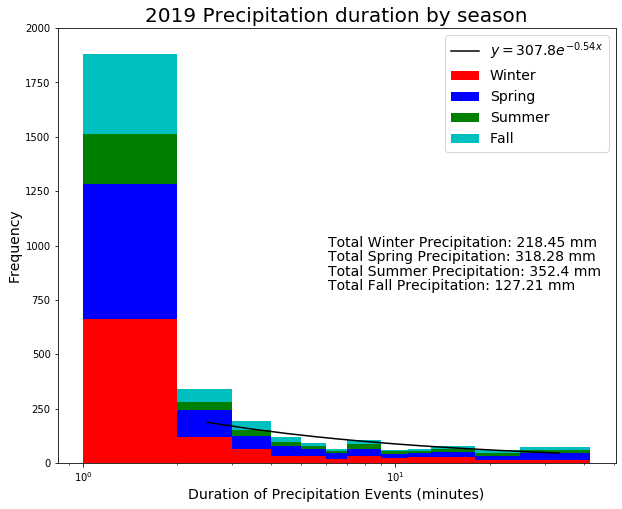
\includegraphics[width=0.675\textwidth]{Figures/More_detail_precip_2019.png}
  \caption[Precipitation histogram for 2019 broken down by
    season]{\label{p2019} Distribution of precipitation duration in
    2019, with a breakdown by seasons. The minimum duration,
    $\tau=1$~min, and the maximum duration over the data set is 368
    min, but the horizontal axis was limited to the 98th percentile of
    the durations, 42~min, for clarity. Superposed is a least-squares
    fit of a line in log-log space of duration versus frequency for
    the entire year, excluding the 1--2~min bin, quoted as the
    equivalent exponential in this space.}
\end{figure}
\begin{figure}[b]
  \centering
  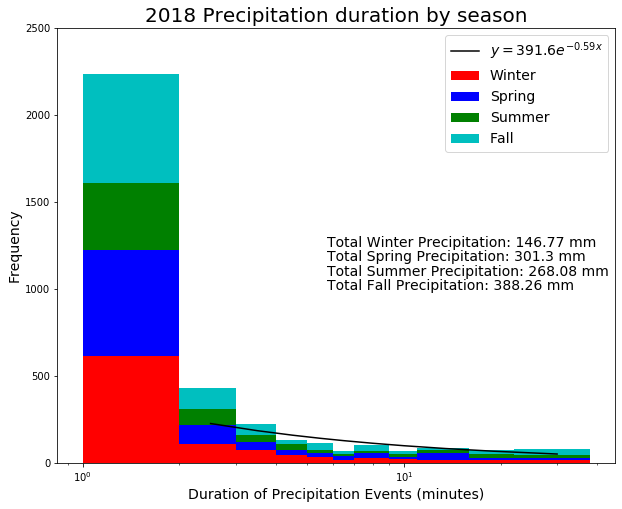
\includegraphics[width=0.675\textwidth]{Figures/precip_2018.png}
  \caption[Precipitation histogram for 2018 broken down by season]{\label{p2018}
    Distribution of precipitation duration in 2018, with a breakdown
    by seasons. The layout is as in Figure~\ref{p2019}.}
\end{figure}
	
\clearpage
\begin{figure}[t]
	\centering
	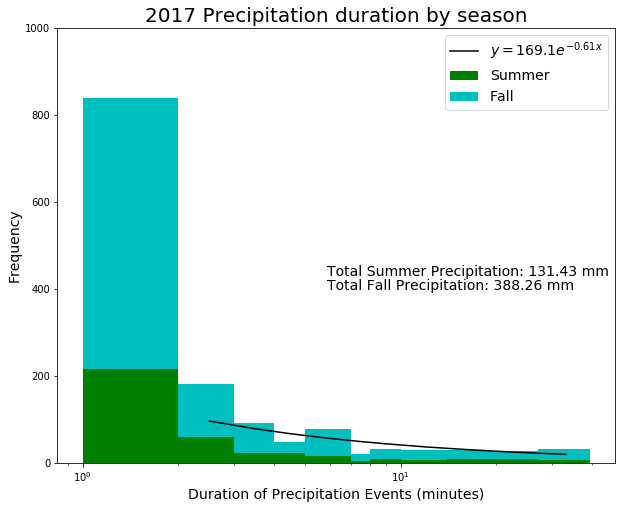
\includegraphics[width=0.675\textwidth]{Figures/precip_2017.png}
	\caption[Precipitation histogram for 2017 broken down by
          season]{\label{p2017} Distribution of precipitation duration
          in 2017, with a breakdown by seasons. The layout is as in
          Figure~\ref{p2019}. Note that data collection began on XX YY
          of this year.}
\end{figure}
\begin{figure}[b]
	\centering
	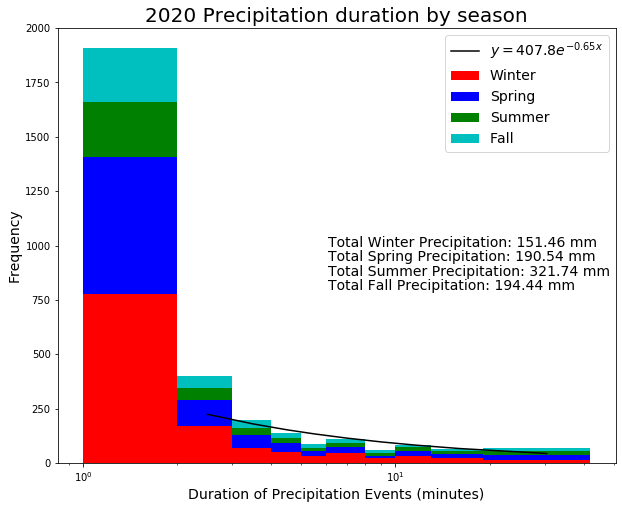
\includegraphics[width=0.675\textwidth]{Figures/precip_2020.png}
	\caption[Precipitation histogram for 2020 broken down by season]{\label{p2020}
		Distribution of precipitation duration in 2020, with a breakdown
		by seasons. The layout is as in Figure~\ref{p2019}.}
\end{figure}

\clearpage
Excluding the first interval shown, focusing on events of duration
greater than or equal to 2 min, we propose an exponential model for
the histogram, with the following equation:
\begin{equation}
  F = \beta e^{\alpha d}
,
\end{equation}
where $F$ is the frequency and $d$ the duration, and with $\beta$ the
unitless frequency coefficient and $\alpha$ is the exponential
coefficient (in units of 1/min). .
	
Is the exponential different for W/S/S/F? Can you tell the difference?
Is the exponential different for different years? Can you tell the
difference?  And what summarizes it all. \\ The following table shows
the coefficients and the exponential coefficients from the looking at
the yearly frequency of precipitation duration. \\
\begin{center}
	\begin{tabular}{l*{3}{c}r}
		\centering
		Year      & $\beta $ & $\alpha$  \\
		\hline
		2017      & 169.1           & -0.61    \\
		2018      & 391.6           & -0.59    \\
		2019      & 307.8           & -0.54   \\
		2020      & 407.8           & -0.65    \\
	\end{tabular}
\end{center}
Based on this table, the $\beta$ values are similar to each other with
the exception of 2017, which only had partial data starting from the
summer. Even, with the partial data we have from 2017 and 2020, it is
clear that the $\alpha$ values are similar to each other. Focusing on
the years with complete data, 2018 and 2019, it is clear that yearly
variations exists between them.  \\ Winter Precipitation coefficients
and exponential coefficients. \\


\begin{center}
	\begin{tabular}{l*{3}{c}r}
		Year      & $\beta $ & $\alpha$  \\
		\hline
		2018      &            &      \\
		2019      &            &    \\
		2020      &             &      \\
	\end{tabular}
\end{center}
Spring Precipitation coefficients and exponential coefficients.\\ 
\begin{center}
	\begin{tabular}{l*{3}{c}r}
		Year      & $\beta $ & $\alpha$  \\
		\hline
		2018      &            &      \\
		2019      &            &    \\
		2020      &             &      \\
	\end{tabular}
\end{center}
Summer Precipitation coefficients and exponential coefficients. \\
\begin{center}
	\begin{tabular}{l*{3}{c}r}
		Year      & $\beta $ & $\alpha$  \\
		\hline
		2017      &            &     \\
		2018      &             &     \\
		2019      &            &    \\
		2020      &             &      \\
	\end{tabular}
\end{center}
Fall Precipitation coefficients and exponential coefficients. \\
\begin{center}
	\begin{tabular}{l*{3}{c}r}
		Year      & $\beta $ & $\alpha$  \\
		\hline
		2017      &            &     \\
		2018      &             &     \\
		2019      &            &    \\
		2020      &             &      \\
	\end{tabular}
\end{center}
\section{Results \label{sec:results}}


\section{Discussion \label{sec:discussion}}


\section{Conclusions \label{sec:conclusions}}


%--References
\small
\renewcommand{\bibsep}{0em}

\renewcommand{\bibname}{References}
\bibliographystyle{Latex/gji}
\bibliography{refs}

\end{document}
